Tässä luvussa esitetään perusteet ja tarvittavat tiedot hyväksymistestauksesta..

\section{Hyväksymistestauksen tarkoitus}

% Teksti tähän

% \section{Testiautomaatio prosessina}

% Testiautomaation prosessiin kuuluu erilaisia artifakteja, joita luodaan testausprosessin eri vaiheissa.
% Eri vaiheita ovat kronologisessa järjestyksessä ovat muun muassa testisuunnitelma, skenaariot, testitapaukset ja seuranta.

\section{Hyväksymistestausvetoinen kehitys}

Hyväksymistestausvetoisen kehityksen (englanniksi: ATDD, acceptance test driven development) tarkoituksena, kuten testausvetoisessakin kehityksessä on toteuttaa ohjelmistotuotannollinen prosessi testaaminen edellä.
Tämä tarkoittaa käytännössä, sitä että ohjelmistokehittäjät laativat ohjelmiston vaatimusten ja suunnitelman mukaisia iteratiivisesti suoritettavia testitapauksia, ennen niitä käyttävän varsinaisen ohjelmakoodin toteuttamista.
Hyväksymistestausvetoisessa kehityksessä luodaan ennen toteutusta tarvittavat ohjelmiston asiakasvaatimuksia palvelevat hyväksymistestit, joiden ohjelmiston on tarkoitus läpäistä.
Tarvittavat ohjelmiston hyväksymistestit suoritetaan iteratiivisesti ohjelmistokehitysprosessin aikana, ja se tarkoittaa käytännössä jatkuvan integraation ottamista käyttöön ohjelmistokehityksessä.
Hyväksysmistestausvetoinen kehitys on erittäin hyödyllinen ohjelmistokehityksessä käytetty menetelmä, sillä kehitysvaiheessa on aina tarkasti tiedossa vastaako ohjelmiston silloinen tila asiakasvaatimuksia ja kuinka hyvin.
Hyväksymistestausvetoisessa kehityksessä toteutettavat hyväksymistestit testaavat ohjelmistoa kokonaisena järjestelmänä tarkoituksenamukaisesti, siten kuten se esiintyy loppukäyttäjille.

\section{Robot Framework}

Robot framework on geneerinen avoimen lähdekoodin testausalusta hyväksymistestaukseen, hyväksymistestausvetoiseen kehitykseen ja robotisten prosessien automaatioon.

\begin{figure}[H]
  \centering
  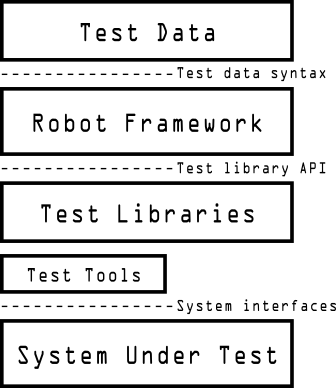
\includegraphics[width=0.4\textwidth]{assets/robot-architecture.png}
  \caption{Robot framework alustan arkkitehtuuri}
  \label{fig:robot-architecture}
\end{figure}

\section{Testitapauksien määrittäminen}

Yleisiä testitapauksien määrittämiseen käytettäviä heuristiikkoja ovat muun muassa:
% \begin{itemize}
%   \item Polut ja tiedostot
%   \item Aika ja päivämäärät
%   \item Numerot
%   \item Merkkijonot
%   \item Yleiset rikkeet
%   \item Muuttujien analyysi
%   \item Kosketuspisteet
%   \item Rajat
%   \item CRUD-toiminnot
%   \item Datan eheys
%   \item Konfiguraatiot
%   \item Katkokset
%   \item Nälkiintyminen
%   \item Samanaikaiset käyttäjät
%   \item Transaktiotulvat
%   \item Riippuvuudet
%   \item Rajaehdot
%   \item Syötetyypit
%   \item Tilan analyysi
%   \item Käyttäjät ja skenaariot
% \end{itemize}

\section{Web-käyttöliittymien erityispiirteet}

Web-käyttöliittymillä on myös omia erityispiirteitä, jotka vaikuttavat testitapauksien laatimiseen.
\begin{itemize}
  \item Navigointi
  \item Syötteet
  \item Syntaksi
  \item Selainasetukset
\end{itemize}

  \subsection{Selenium}

  % Teksti tähän

  \subsection{Moni-selaimellinen testaus}

  % Teksti tähän

\section{Priorisointiongelma}

Testitapauksien priorisointi on kustannussyistä tai resurssien optimoinnin kannalta erittäin tärkeää.
Ohjelmistotestauksessa on hyvä tiedostaa, että ohjelmistotuotetta ei usein voida testata täydellisesti, joka nostaa esiin tarpeen tärkeimpien testitapauksien löytämisestä.
Testitapauksia voidaan priorisoida monella tavalla, joihin tämä diplomityö tuo yhden uudenlaisen painottua verkkoa hyödyntävän lähestymistavan.
\begin{itemize}
  \item Painotetun verkon hyödyntäminen
  \item Muut priorisointitavat
\end{itemize}